\section{The Sort Operator}
\label{sort}

Sorting is among the most commonly used operations in database systems,
forming the core of operators such as \emph{merge-join}, \emph{order-by} and
some flavors of \emph{group-by}.  The process of sorting is quite
write-intensive since the commonly used in-memory sorting algorithms,
such as \textit{quicksort}, involve considerable data movement. In the
single pivot quicksort algorithm with $n$ elements, the average number
of swaps is of the order of $0.3nln(n)$~\cite{swaps}. There are other
algorithms such as \emph{selection sort} which involve much less data
movement, but they incur \emph{quadratic} time complexity in the number
of elements to be sorted, and are therefore unsuitable for large datasets.

In the following sections, we begin with the analysis of the conventional
quicksort algorithm. Later, we propose a modified \emph{in-place} sorting algorithm termed
\emph{multi-pivot quicksort}, which improves upon conventional quicksort
to achieve a reduction in PCM writes, by trading expensive writes for 
additional reads.

\subsection{Conventional Quicksort}
The conventional quicksort algorithm begins by choosing one of the
input elements as a pivot. Each pass divides the input array into two
partitions, one containing elements less than the pivot, and the other
containing those that are greater. This is achieved by means of in-place
swapping of elements in the array. This partitioning is done recursively
for the obtained partitions to give the final sorted array.

If the initial array is much larger than the DRAM size, it would
entail evictions from the DRAM during the swapping process of
partitioning. These evictions might lead to PCM writes if the evicted
DRAM lines are \textit{dirty}, which is likely since elements are being
swapped. If the resulting partition sizes continue to be larger than
DRAM, partitioning them in turn will again cause DRAM evictions and
consequent writes. Clearly, this trend of writes will continue in the
recursion tree until the partition sizes become small enough to fit within
DRAM. Thereafter, there would be no further evictions during swapping
and the entire subsequent sorting process would finish within the DRAM.

\begin{comment}
\begin{figure}
\centering
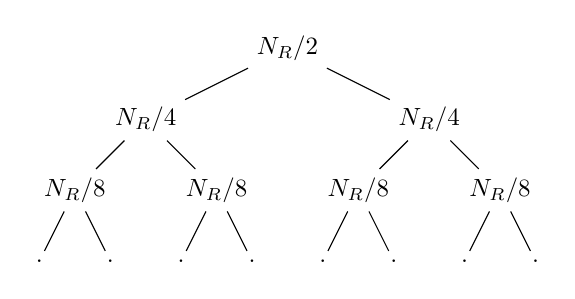
\begin{tikzpicture}[scale=.9, transform shape]

\tikzstyle{every node} = [rectangle, fill=gray!0]

\node (s) at (1,0) {.};
\node (t) at (2,0) {.};
\node (u) at (3,0) {.};
\node (v) at (4,0) {.};
\node (w) at (5,0) {.};
\node (x) at (6,0) {.};
\node (y) at (7,0) {.};
\node (z) at (8,0) {.};

\node (a) at (1.5,1) {$N_R$/8};
\node (b) at (3.5,1) {$N_R$/8};
\node (c) at (5.5,1) {$N_R$/8};
\node (d) at (7.5,1) {$N_R$/8};

\node (e) at (2.5,2) {$N_R$/4};
\node (f) at (6.5,2) {$N_R$/4};

\node (g) at (4.5,3) {$N_R$/2};

\draw[-] (s) -- (a);
\draw[-] (t) -- (a);
\draw[-] (u) -- (b);
\draw[-] (v) -- (b);
\draw[-] (w) -- (c);
\draw[-] (x) -- (c);
\draw[-] (y) -- (d);
\draw[-] (z) -- (d);

\draw[-] (a) -- (e);
\draw[-] (b) -- (e);
\draw[-] (c) -- (f);
\draw[-] (d) -- (f);

\draw[-] (e) -- (g);
\draw[-] (f) -- (g);
\end{tikzpicture} 
\caption{Recursion tree for quicksort swaps}
\label{fig:rec_tree}
\end{figure}
\end{comment}

\textbf{PCM write analysis:} 
Given an array with randomly permuted $N_R$ tuples, let us assume the
chosen pivot in each phase of recursion is the median of the partition
tuples. Since the tuples are arranged randomly, the probability that
the tuples is in the right partition is $1/2$. In other words, $N_R/2$
tuples are expected to be incorrectly placed.

In the next level of the recursion tree, there will be about $N_R/4$
incorrectly placed tuples for both the partitions, again totalling to
$N_R/2$. This total of $N_R/2$ tuples would continue at each level of the
recursion tree. % as shown in Figure~\ref{fig:rec_tree}.

If Hoare partitioning~\cite{cormen} is used, wherein each misplaced
element is swapped with another misplaced element in the opposite
partition, moving the elements to their right partitions will incur $N_R/2
\times L_R$ writes at each level. This trend of writes will continue
until the size of the partition reaches to less than $D$, i.e. when the
level $l = \lceil log_2 (\frac{N_R L_R}{D}) \rceil$. Post this, there
would be a total of $N_R L_R$ writes incurred when all the individual
partitions are sorted within DRAM and written out. Hence, we
obtain the total writes as:
\begin{equation}
\label{eq:sort_conv}
\begin{split}
%W_{sort\_conv} = \sum\limit_l (N_R/2 \times L_R) + N_R L_R\\
W_{sort\_conv} = \sum_l (N_R/2 \times L_R) + N_R L_R\\
= 0.5N_RL_R \lceil log_2(\frac{N_R L_R}{D}) \rceil + N_R L_R\\
  = N_RL_R (0.5 \lceil log_2(\frac{N_R L_R}{D}) \rceil + 1) \\
\end{split}
\end{equation}



\begin{comment}
In the quicksort algorithm on randomly permuted $N_R$ tuples, the average number of swaps is $0.33N_Rln(N_R)$ \cite{swaps}. If each pair of swapped tuples gets evicted from DRAM to PCM after each intermediate swap, there will be two tuple writes (of $L_R$ bytes each) in PCM per pair of swapped tuples. Hence, the total number of writes is given by:  
\end{comment}

\subsection{PCM-conscious multi-pivot quicksort}
\label{subsec:sort_mpivot}
From the above discussion, it is clear that the faster we converge to
partition sizes within DRAM size, the better. Due to use of a single
pivot, conventional quicksort is restricted to just two partitions in each
recursive step. Therefore, we now propose a \emph{multi-pivot} implementation of
quicksort instead, with the expectation that this would help in getting the
individual partitions more quickly to a size within the DRAM capacity.

A hurdle, however, that arises in the multi-pivot case, is that we do
not have any prior information about the boundaries of the partitions.
This hampers the direct movement of elements to their respective
partitions during the partitioning step. We address this limitation
by adding a separate \textit{read phase} that makes an initial read
pass over the input elements, counting the number of elements between
each consecutive pair of pivots. Note that these counters, by virtue
of being continuously updated during the read pass, are likely to be
updated \emph{within DRAM itself}, not incurring PCM writes.

The boundary information obtained in the read phase is used in
a subsequent \emph{swap phase} to move the tuples to the right
partitions. Finally, the \emph{sort phase} sorts each partition
separately. These phases are explained in detail below.

\subsubsection{Read Phase} 
In the read phase, we divide the input relation into $p$ partitions,
where $p = \lceil \frac{N_R L_R}{D} \rceil$, using $p-1$ random tuples
as pivots.  Since the pivots are picked at random, the hope is that each
partition is approximately of size $D$.  These pivots are then copied
to a separate location and sorted. Subsequently, we scan through the
array of tuples in the relation, counting the number of elements between
each consecutive pair of pivots. This is accomplished by carrying out, for each
tuple in the array, a binary search within the sorted list of pivots.

In spite of the random choice of pivot values, it is quite possible that
some partitions may turn out to be larger than the DRAM. We account
for this possibility by conservatively creating a larger number of
initial partitions. Specificially, the number of partitions is $p =
\lceil c \times \frac{N_R L_R}{D} \rceil$, where $c \geq 1$ is a design
parameter. In our experience, setting $c = 2$ worked well in practice.
Subsequently, we consider each pair of adjoining partitions and coalesce
them if their total size is within the DRAM size, after leaving some space
for bookkeeping information. 

While the above heuristic approach is quite effective, it still does not
guarantee that all the resultant partitions will be less than DRAM size. The
(hopefully few) cases of larger-sized partitions are subsequently handled
during the sort phase.

The pseudo-code for the read phase is outlined in
Algorithm~\ref{alg:read_phase}.

\begin{algorithm}
\small
\caption{Read Phase}
\label{alg:read_phase}
\textbf{array[]} is the array of input tuples\\
\textbf{c} is a design parameter $\geq 1$\\
\begin{algorithmic}[1]
\State p = $\lceil c\times \frac{N_R L_R}{D} \rceil$
\State randIndex[] = generate $p-1$ random indexes
\State pivot[] = array[randIndex];
\State sort(pivot[])
\State size[] = {0...0}   
\Comment{size of sub-arrays}
\For {i=$1$ to $N_R$}
\State partition = getPartition(array[i]) 
\State size[partition]++ 
\EndFor
\Comment {Time complexity=$N_R\times log_2p$ }
\State cumulative = 0
\For {i=$1$ to $p$}
\State cumulative = cumulative + size[i]
\State partitionStart[i+1] = cumulative
\EndFor
\Comment {Time complexity=$p$ }
\State return partitionStart[]
\end{algorithmic}

\end{algorithm}


\subsubsection{Swap Phase} 
The swap phase uses the information gathered in the read phase to group
tuples of the same partition together. The algorithm first picks up
a wrongly placed entry $a$ in a partition $P_x$, and determines its
correct partition $P_a$ by comparing it with the pivots. It then finds
another wrongly placed entry $b$ belonging to partition $P_a$, and writes
$a$ in its place. Now the correct partition $P_b$ of $b$ is determined
and a misplaced element $c$ is identified from $P_b$ as a victim for
replacement. The algorithm proceeds in the same manner till the cycle
completes with the last incorrectly placed entry belonging to partition
$P_x$. Such replacement cycles are repeatedly initiated until all
elements are placed in their correct partitions. This is similar in
flavor to the classical cycle-sort algorithm \cite{cycle_sort}.

The pseudo-code for the swap phase is shown in
Algorithm~\ref{alg:swap_phase}.  The maximum number of writes is bounded
by $N_R L_R$, corresponding to the worst case where \emph{every} tuple
has to be moved to its correct partition.

\begin{algorithm}[h!]
\small
\caption{Swap Phase}
\label{alg:swap_phase}
\textbf{partitionStart[]} is obtained from Read Phase\\
\textbf{nextUnresolvedIndex[]} indicates the next position to be examined for each partition\\
\begin{algorithmic}[1]
\State nextUnresolvedIndex[] = partitionStart[]
\For {i=1 to $N_R$}
	\State curPartitionCorrect = getPartition(array[i])
     \If {i between partitionStart[curPartitionCorrect] and  partitionStart[curPartitionCorrect+1]}                
     \State nextUnresolvedIndex[curPartitionCorrect] = i+1
	\State continue;
     \Else
     		\State firstCandidateLoc = i
			\State presentCandidate = array[i]             
            \State flag = 1;
            \While {flag} 
                \State targetPartitionStart = nextUnresolvedIndex[curPartitionCorrect];
                \State targetPartitionEnd = partitionStart[curPartitionCorrect + 1];
                \For {k=targetPartitionStart to targetPartitionEnd} 
                \State nextPartitionCorrect = getPartition(array[i]);
                    \If {k between partitionStart[nextPartitionCorrect]                       and 
                    \State partitionStart[nextPartitionCorrect + 1]}
                        \State continue;
                        
                    \ElsIf {k == firstCandidateLoc} 
                        \State flag = 0; \Comment Indicates it is a cycle
                    \EndIf
                    \State swap(presentCandidate, array[k]);
                    \State nextUnresolvedIndex[curPartitionCorrect] = k+1;
                    \State curPartitionCorrect = nextPartitionCorrect
                    
                    \State break;
             
				\EndFor
			\EndWhile
	\EndIf
\EndFor
\Comment {Time complexity=$N_R\times log_2p$ }
\end{algorithmic}

\end{algorithm}


\subsubsection{Sort Phase}
Finally, each of the partitions are sorted separately using conventional
quicksort to get the final PCM sorted array. For partitions that turn
out to be within the DRAM size, the sort phase is completed using
conventional quicksort fully within the DRAM, and not causing any
intermediate evictions to PCM.  On the other hand, if some larger-sized
partitions still remain, we recursively apply the multi-pivot quicksort
algorithm to sort them until all the resulting partitions fit within DRAM 
and can be internally sorted.

\begin{algorithm}
\small
\caption{Sort Phase}
\label{alg:sort_phase}
\begin{algorithmic}[1]
\For {i=1 to p}
\If {size[p] $<$ D}
\State quicksort (partition p)
\Else 
\State multi-pivot quicksort (partition p)
\EndIf 
\EndFor
\end{algorithmic}

\end{algorithm}

Figure~\ref{fig:mpsort} visually displays the steps involved in the
multi-pivot quicksort of an array of nine values. First, in the read phase,
$30$ and $15$ are randomly chosen as the pivots. These pivots divide the input
elements into 3 different ranges: ($< 15$), ($\geq 15$, $< 30$), ($\geq
30$). The count of elements in each of these ranges is then determined by
making a pass over the entire array -- in the example shown, three elements
are present in each partition.  Then, in the swap phase, the elements are
moved to within the boundaries of their respective partitions. Finally,
in the sort phase, each partition is separately sorted within the DRAM.


%\newcolumntype{b}{>{\columncolor{white}}c}
\begin{figure}[h]
	\centering
	\subfloat[Read Phase]{	
  	%\includegraphics[width=8cm]{sort_step_1.png}
  	
  	\begin{tabular}{|c|c|c|y|c|y|c|c|c|}
        \hline
        24&3&33&30&21&15&7&32&11\\\hline
    \end{tabular}
    }
	\hspace{0mm}
	\subfloat[Swap Phase]{
  	\begin{tabular}{|x|x|x|y|y|y|z|z|z|}
        \hline
        7&3&11&24&21&15&30&32&33\\\hline
    \end{tabular}
    }
    \hspace{0mm}
	\subfloat[Sort Phase]{
  	\begin{tabular}{|x|x|x|y|y|y|z|z|z|}
        \hline
        3&7&11&15&21&24&30&32&33\\\hline
    \end{tabular}
    }
	\caption{Multi-Pivot Sort}
	\label{fig:mpsort}
	
\end{figure}
\textbf{PCM write analysis}: Though the partition boundary counters
are continuously updated during the Read phase, they are expected to
incur very few PCM writes. This is because since all those updates are
in quick succession, the counters are unlikely to be evicted from DRAM
\emph{during} the update process. Similarly, negligible writes would
be incurred during the copying and sorting of the pivots. During the
Swap phase, there will be no more than $N_R L_R$ writes since each tuple is written
at most once while placing it within its partition boundaries. If each
partition is within the DRAM size, the Sort phase (for each partition)
will finish within DRAM and there will be another $N_R L_R$ writes upon
eventual eviction of sorted partitions to PCM. 

In the above, we are assuming the best case for partitioning wherein all the
initial partitions fit into DRAM, and the worst case for swapping wherein
all tuples have to be moved to new partitions. Our expectation is that these
effects will on average balance each other out, and therefore the total writes is
estimated by
\begin{equation}
\label{eq:mpivot}
  W_{mpivot} = 2N_RL_R
\end{equation}









\begin{comment}
\subsection{Multi-pivot sort without explicit partitioning}
The multi-pivot algorithm discussed in the previous section incurred $N_R L_R$ writes during the swap phase due to materialization of partitions in-place. If the available PCM size is sufficient to accommodate another copy of the array to be sorted, we can avoid partitioning writes by trading the swap phase for multiple \textit{sort} passes, each pass carrying out the sorting one of the partitions in the array using the additional space available. This space eventually feeds the sorted tuples as input to the parent operator in the query plan tree. 

In each pass, we go over the entire array, copying the elements belonging to one partition to the space and subsequently sort them there, before moving to the next partition. The process of copying would seem to incur writes of itself and would thus apparently be self-defeating. However, in this case, we leverage the DRAM replacement policy by choosing an appropriate partition size which would prevent dirty (written) words from getting evicted. For N-Chance replacement policy, such a partition size would be $\frac{(N-1)}{K}\times D$. This would ensure that the extracted partition elements do not get evicted before sorting finishes for the partition. In this manner, each partition is processed sequentially by making multiple passes over the entire input array.

\textbf{PCM write analysis}: In this scheme, since there are no extraction writes, the writes incurred are just due to the eviction of the sorted partitions from DRAM. Thus the total writes are given by 
\begin{equation}\label{eq:mpivot_wep}
  W_{mpivot\_wep} = N_RL_R
\end{equation}
\end{comment}
